%# -*- coding: utf-8 -*-
% stars.tex
% asymptotebyexample 的一章,数组、函数和随机数等内容

\chapter{令狐庸的星空图}
\label{chap:stars}

令狐庸是大学概率统计专业的学生,因为酷爱金庸的武侠小说,便给自己起了个“令狐
庸”的网名。这日他读到《天龙八部》的一段:
\begin{quotation}
\itshape
阿朱道:“本来我不知道,看到阿紫肩头刺的字才知。她还有一个金锁片,跟我那个金
锁片,也是一样的,上面也铸着十二个字。她的字是:‘湖边竹,盈盈绿,报平安,多
喜乐。’我锁片上的字是:‘天上星,亮晶晶,永灿烂,长安宁。’我……我从前不知
道是什么意思,只道是好口采,却原来嵌着我妈妈的名字。我妈妈便是那女子阮……阮
星竹。这对锁片,是我爹爹送给我妈妈的,她生了我姊妹俩,给我们一个人一个,带在
颈里。”
\end{quotation}
便打算把“天上星,亮晶晶,永灿烂,长安宁”这几句画成一幅插图。最近他在学习
\Asy{},尽管他清楚这种工作应该使用 Inkscape 之类的图形界面软件来做,但本来艺
术修养不高的他还是决定直接用 \Asy{} 编程画图。

令狐庸心目中的插图就像\autoref{fig:stars} 一样。
\begin{figure}[htpb]
  \centering
  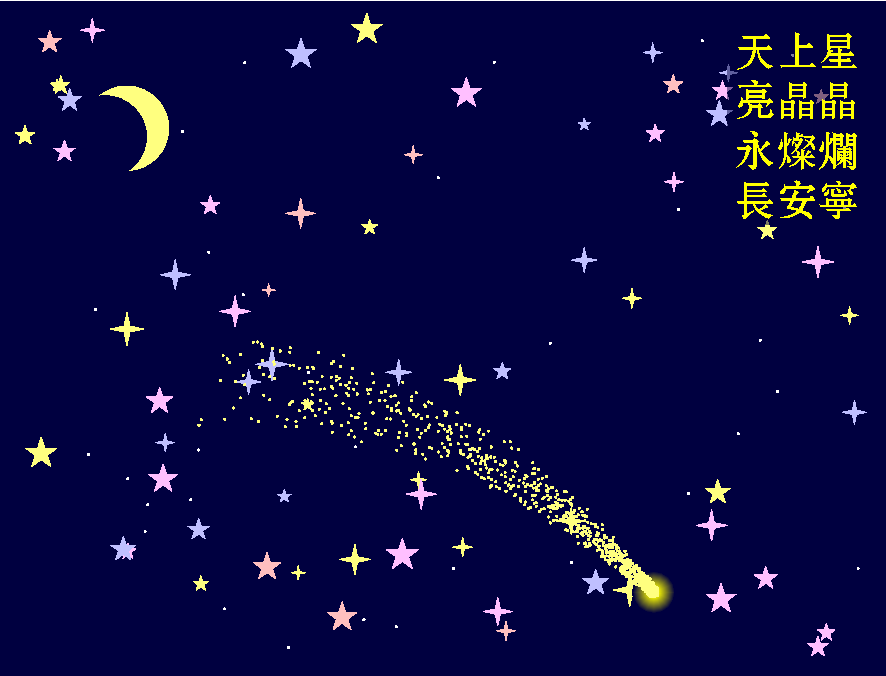
\includegraphics{stars.pdf}
  \caption{令狐庸理想中的星空图}
  \label{fig:stars}
\end{figure}

在他设想的图中,主体是深蓝色的夜空,空中有一弯月亮,有无数星星,还有一颗巨大
的彗星。尽管艺术感并不强,但这幅图看起来相当复杂而且杂乱无章,对于初学 \Asy{}
不久的令狐庸来说,也算是一种挑战了。

\section{在循环中构造路向}
\label{sec:guideinloop}

星空图中最基本的元素就是星星。令狐庸的第一件事就是画出星星。简单的星星就是一
个小圆点,但真正让令狐庸头疼的是四角星、五角星之类的形状。更进一步,令狐庸想
搞明白的是,如何画出一般的星形。

令狐庸的数学不错,一个自然的想法是,把星形的每个角上的点坐标计算出来,依次连
接得到整个星形的路径。而 $n$ 角星形共有 $2n$ 个点,其中 $n$ 个是外面的角点,
$n$ 个是内凹的角点,外面的 $n$ 个点与里面的 $n$ 个点分别都在以星形中心的两个
圆上均匀分布,如\autoref{fig:5star} 所示。
\begin{figure}[H]
  \centering
\begin{asy}
import markers;
picture star(int n)
{
    picture pic;
    size(pic, 0, 8cm);
    guide g;
    real theta=180/n;
    real r = Cos(2theta)/Cos(theta);
    for (int i = 0; i < n; ++i)
        g = g -- dir(90+2theta*i) -- r*dir(90+theta+2theta*i);
    g = g -- cycle;
    filldraw(pic, g, paleblue, linewidth(2bp));
    pair o = (0,0), a = (0,1), b = r*dir(90+theta), d = r*dir(90+3theta);
    draw(pic, Label("$R$",1/3), o -- a, darkblue+2bp);
    draw(pic, Label("$r$",LeftSide), o -- b, darkgreen+2bp);
    draw(pic, b -- d, gray+2bp);
    markangle(pic, "$\theta$", radius=18bp, a, o, b);
    return pic;
}
add(star(5).fit());
\end{asy}
  \caption{$n=5$ 时的星形}
  \label{fig:5star}
\end{figure}
其中,从中心点到 $n$ 角星形的相邻角点(一凸一凹)的夹角容易得到:
\[
  \theta = \frac{360^\circ}{2n} = \frac{180^\circ}{n}.
\]
设大圆半径是 $R$,则只要求出小圆半径 $r$,则整个 $n$ 角星形的各点坐标就很容
易得到了。这里,星形的形状要求是相隔一个角的两角的边共线(见%
\autoref{fig:5star} 中的灰色线)。

下面,就是考验令狐庸几何计算能力的时候了。他在图上添加了几条辅助线,问题立即
变得清晰起来:
\begin{figure}[H]
  \centering
\begin{asy}
import markers;
picture star(int n)
{
    picture pic;
    size(pic, 0, 8cm);
    // draw star
    guide g;
    real theta=180/n;
    real r = Cos(2theta)/Cos(theta);
    for (int i = 0; i < n; ++i)
        g = g -- dir(90+2theta*i) -- r*dir(90+theta+2theta*i);
    g = g -- cycle;
    filldraw(pic, g, paleblue, linewidth(2bp));
    // markers
    pair o = (0,0), a = (0,1), b = r*dir(90+theta),
         c = dir(90+4theta), d = r*dir(90+3theta);
    draw(pic, Label("$R$",1/3), o -- a, darkblue+2bp);
    draw(pic, Label("$r$",LeftSide), o -- b, darkgreen+2bp);
    draw(pic, o -- c ^^ b -- d, gray+2bp);
    markangle(pic, "$\theta$", radius=18bp, a, o, b);
    markangle(pic, "$\alpha$", b, a, o);
    markangle(pic, "$\beta$", radius=8bp, o, b, a);
    dot(pic, Label("$O$",align=SE), o);
    dot(pic, Label("$A$",align=N), a);
    dot(pic, Label("$B$",align=NW), b);
    dot(pic, Label("$C$",align=W), c);
    dot(pic, Label("$D$",align=WSW), d);
    return pic;
}
add(star(5).fit(), 0, align=10W);
add(star(6).fit(), 0, align=10E);
\end{asy}
  \caption{$n=5$, $6$ 时的星形分析}
  \label{fig:56star}
\end{figure}
如\autoref{fig:56star} 所示,星形满足 $A$, $B$, $D$, $C$ 四点共线的条件。在等
腰三角形 $AOC$ 中,容易看出 $\angle AOC = 4\theta$,从而
\[
  \alpha = (180^\circ-\angle AOC)/2 = 90^\circ - 2\theta.
\]
于是在三角形 $AOB$ 中即有
\[
  \beta = 180^\circ - \theta - \alpha = 90^\circ +\theta.
\]
于是,利用正弦定理
\[
  \frac{r}{\sin \alpha} = \frac{R}{\sin \beta}
\]
即得
\begin{align*}
  r &= \frac{\sin\alpha}{\sin\beta} R \\
    &= \frac{\sin\left( 90^\circ -2\theta \right)}
            {\sin\left( 90^\circ +\theta \right)} R \\
    &= \frac{\cos 2\theta}{\cos \theta} R.
\end{align*}

现在令狐庸已经成功地算出了 $n$, $\theta$, $R$, $r$ 的关系式,于是 $n$ 角星上
的任一个点都容易算出。不妨设 $R = 1$,利用 \Asy{} 的 |dir| 函数,则容易在
\Asy{} 中计算出 $n = 5$ 时 $A$, $B$ 两点的坐标:
\begin{asycode}
int n = 5;
real theta = 180 / n;
real r = Cos(2theta) / Cos(theta);
pair a = dir(90);
pair b = r * dir(90+theta);
\end{asycode}
而五角星上的其他点就可以直接由 $A$, $B$ 两点坐标绕原点旋转 $2\theta$ 的整数倍
得到,再注意到 $A$, $B$ 都是由 |dir| 函数的倍数定义的,所以这个旋转变换可以直
接写进 |dir| 函数的参数,即 |dir(90+i*2theta)|, |r*dir(90+theta+i*2theta)|(%
|i| 取 $0$, $1$, $2$, \ldots, $n-1$)。

现在,令狐庸已经得到所有的点坐标,剩下的问题就是把这些点连接为星形的路向。$n$
角星形的路向是由 $n$ 组相同的点连接得到的,很自然地,就可以使用循环语句来逐步
地构造路向:
\begin{asycode}
int n = 5;          // `\color{comment}五角星`
real theta = 180 / n;
real r = Cos(2theta) / Cos(theta);
guide unitstar;     // `\color{comment}外圈半径为 1 的星形路向,初值为空`
// `\color{comment}在循环中连接所有的点`
for (int i = 0; i < n; ++i)
    unitstar = unitstar -- dir(90+i*2theta) -- r*dir(90+theta+i*2theta);
// `\color{comment}连接星形路向的起末点,构成闭路向`
unitstar = unitstar -- cycle;

// `\color{comment}测试`
size(5cm);
filldraw(unitstar, lightblue, gray+2mm);
\end{asycode}
\begin{figure}[H]
  \centering
\begin{asy}
int n = 5;
real theta = 180 / n;
real r = Cos(2theta) / Cos(theta);
guide unitstar;
for (int i = 0; i < n; ++i)
    unitstar = unitstar -- dir(90+i*2theta) -- r*dir(90+theta+i*2theta);
unitstar = unitstar -- cycle;
size(5cm);
filldraw(unitstar, lightblue, gray+2mm);
\end{asy}
\end{figure}
哈,一个五角星就这样画成了。而且只要把上面代码中的 $n$ 改为 $6$,就可以得到六
角星了:
\begin{figure}[H]
  \centering
\begin{asy}
int n = 6;
real theta = 180 / n;
real r = Cos(2theta) / Cos(theta);
guide unitstar;
for (int i = 0; i < n; ++i)
    unitstar = unitstar -- dir(90+i*2theta) -- r*dir(90+theta+i*2theta);
unitstar = unitstar -- cycle;
size(5cm);
filldraw(unitstar, lightblue, gray+2mm);
\end{asy}
\end{figure}

星形令狐庸已经可以画好,可整幅插画看起来却还是遥遥无期。如何把不同类型的星形
统一起来,如何把星形均匀而又随机地放在图中,尤其是那个看起来十分复杂的彗星,
现在成为令狐庸案头的新的难题。

\section{自定义函数}
\label{sec:function}

\index{函数}
在 \autoref{sec:guideinloop} 中已经得到了五角星、六角星以至 $n$ 角星的画法。
不过,令狐庸发现,如果需要同时使用各种不同的星形,就不得不重复书写构造星形路
向的代码——但这些代码除了 |n| 的取值外是完全一样的。这就需要使用 \Asy{} 的函
数定义,把构造星形路向的过程进行抽象。令狐庸这样定义他的函数:
\begin{asycode}
// `\color{comment}返回半径为 1 的星形路向`
guide star(int n)
{
    real theta = 180 / n;
    real r = Cos(2theta) / Cos(theta);
    guide unitstar;
    for (int i = 0; i < n; ++i)
        unitstar = unitstar -- dir(90+i*2theta) -- r*dir(90+theta+i*2theta);
    unitstar = unitstar -- cycle;
    return unitstar;
}
\end{asycode}
于是要画一个五角星,只需要再用
\begin{asycode}
size(5cm);
draw(star(5));
\end{asycode}
调用这个函数即可。\index{函数!调用}而同时画五角星和六角星也可以方便地做到:
\begin{asycode}
size(5cm);
draw(star(5));
draw(shift(2) * star(6));
\end{asycode}

\index{函数!定义}
\index{函数!原型}\index{函数!体}
函数的定义分成两个部分:函数原型和函数体。在上面星形路向的函数中,函数原型部
分是
\begin{asycode}
guide star(int n)
\end{asycode}
它表示一个名字是 |star| 的函数,接受一个 |int| 类型名为 |n| 的整数参数,返回
值的类型是 |guide|(路向)。而后面括在花括号中的部分则是函数体,表示整个函数
进行的操作。在函数体中可以使用在函数原型中声明的所有参变量,就如同这些变量是
在函数体中定义的一样。在函数体的最后一句通常是一个 |return|
\index{return@\asyinline=return=} 语句,它将退出整个函数的运行,并把 |return|
语句后面的表达式作为这个函数的返回值。\index{函数!返回值}一般地,函数的定义形
如:
\index{函数!参数}
\begin{asycode}
`返回类型` `函数名`(`参数类型$_1$` `参数$_1$`, `参数类型$_2$` `参数$_2$`, ……)
{
    `各种语句`
    return `返回值`;
}
\end{asycode}
在函数体的内部是一个独立的环境(叫做作用域\index{作用域}),函数的参数和函数
体内新定义的变量都只在函数体内部这个作用域有效,而不会影响作用域之外的内容。
这就使得代码可以分成函数一块一块互不影响地分别设计,而不必担心在这里的变量
|n| 会不会影响别处的另一个变量 |n|。

函数定义的这些部分并不都是必需的。函数可以没有参数,此时函数只相当于给一段语
句的集合起一个名字。没有参数的函数较少使用,通常这种函数都会使用在函数体外定
义的变量来产生不同的行为,例如后面 \autoref{sec:randomarray} 将提到的伪随机数
函数 |rand()|。更常见的情况是没有返回值的函数,此时函数体就不需要有 |return|
语句(或者使用一个没有值的 |return| 语句表示退出函数),但仍然需要声明函数的
返回类型为 |void|\index{void@\asyinline=void=}——即空类型\index{空类型}。和
数学中的函数不同,\Asy{} 中一个函数有用不仅因为它可以计算出一个返回值,还在于
它能进行许多操作,比如画图。所以令狐庸写了这样一个画星形的函数:
\begin{asycode}
void drawstar(int n, pen drawpen)
{
    draw(star(n), drawpen);
}
\end{asycode}
这样,|drawstar(7, red)| 就可以画出一个红色的七角星。

\index{函数!默认参数}
\index{函数!缺省参数|see{默认参数}}
像在 C++ 中一样,在定义函数时,函数原型中函数参数还可以有一个默认值,这样调用
函数的时候就可以省略这个参数。例如,令狐庸的画星形函数可以改为
\begin{asycode}
void drawstar(int n = 5, pen drawpen = currentpen)  // currentpen `\color{comment}是当前画笔`
{
    draw(star(n), drawpen);
}
\end{asycode}
于是,如果没有改变当前画笔,只要用 |drawstar()| 就可以画出一个黑色的五角星轮
廓;而用 |drawstar(red)| 则画出红色五角星;用 |drawstar(6)| 画出黑色六角星
\footnote{C++ 的参数可以有缺省值,但允许从最后一个参数开始从后向前省略,不能
这样跳跃缺省参数值。这是因为 C++ 是按位置解析参数的,但 \Asy{} 则还会考虑参数
的类型。注意这个例子中 \asyinline=drawpen(red, 7)= 的形式是不成立的。};用
|drawstar(7, red)| 画出红色七角星。

调用函数时,除了直接写出参数值,还有一种在 \autoref{sec:linedraw} 中就使用过
的一种方式,即用 $\text{键}=\text{值}$ 的方式书写参数,这样即使与函数原型中参
数声明的顺序不同,也可以正确调用,如用 |drawstar(drawpen = red, n = 7)| 画出
红色七角星——这也是 C++ 中不具备的一种语法。

事实上,与数值、画笔等类型一样,函数也是一种数据类型。函数的类型名就是函数原
型去掉函数名字的部分,如正弦函数 |real sin(real x)|
\index{sin@\asyinline=sin=} 的类型就是 |real (real x)| (在不混淆时或可简写为
|real (real)|)。定义一个函数就是定义这个类型的一个变量。因此,一个函数也可以
作为另一个函数的参数,例如在 \Asy{} 绘制函数图形的基本模块 \prgname{graph}
\index{graph 模块@\prgname{graph} 模块} 中,就有函数(这里省略了一些有默认值
的参数):
\index{函数!函数作为参数}
\index{graph@\asyinline=graph=}
\begin{asycode}
guide graph(real f(real), real a, real b);
\end{asycode}
因而可以用
\begin{asycode}
import graph;
size(5cm);
draw(graph(sin, 0, 2pi));
\end{asycode}
画出正弦函数的图像来:
\begin{figure}[H]
  \centering
\begin{asy}
import graph;
size(5cm);
draw(graph(sin, 0, 2pi));
\end{asy}
\end{figure}

因为函数也是一种数据类型,所以一个函数并不必须有名字。使用 |new|
\index{new@\asyinline=new=} 表达式可以构造匿名函数\index{函数!匿名函数}。如计
算 $f(x) = x^2$ 的函数:
\begin{asycode}
new real (real x)  { return x^2; }
\end{asycode}
匿名函数可以直接求值或赋给一个函数变量名,但这都没有什么实际意义:
\begin{asycode}
(new real (real x)  { return x^2; })(5);    // `\color{comment}直接求值得 25`
real f(real x) = new real (real x)  { return x^2; };    `\color{comment}// 赋值`
\end{asycode}
匿名函数实际的作用,是在调用另一函数时作为参数传递,或作为另一函数的返回值。
例如,要画出 $f(x) = x^2$ 的函数图像,就可以用:
\begin{asycode}
import graph;
size(5cm);
draw(graph(new real(real x) {return x^2;}, -1, 1));
\end{asycode}
\begin{figure}[H]
  \centering
\begin{asy}
import graph;
size(5cm);
draw(graph(new real(real x) {return x^2;}, -1, 1));
\end{asy}
\end{figure}

唔,现在回到令狐庸的星星。数学的分析方法很有效,五角星甚至六角星的画法都解决
了,可令狐庸现在还需要四角星:
\begin{figure}[H]
  \centering
\begin{asy}
guide star(int n = 5, real r = 0, real angle = 90)
{
    guide unitstar;
    if (n < 2) return nullpath;
    real theta = 180/n;
    if (r == 0) {
        if (n < 5)
            r = 1/4;
        else
            r = Cos(2theta) / Cos(theta);
    }
    for (int k = 0; k < n; ++k)
        unitstar = unitstar -- dir(angle+2k*theta) -- r * dir(angle+(2k+1)*theta);
    unitstar = unitstar -- cycle;
    return unitstar;
}
size(3cm);
filldraw(star(4), lightblue, linewidth(2));
\end{asy}
\end{figure}
但四角星根本没有任何角的边共线,内圆的半径也就不可能用前面的几何分析得到。此
时,就必须单独给四角星设定半径。另外,令狐庸还想要四角星并不是“正”的(一个
角向正上方向),也需要设定一个初始的角度。因此,经过反复修改,令狐庸最后写出
了这样的函数:
\begin{asycode}
guide star(int n = 5, real r = 0, real angle = 90)
{
    guide unitstar;
    if (n < 2) return nullpath;
    real theta = 180/n;
    if (r == 0) {
        if (n < 5)
            r = 1/4;
        else
            r = Cos(2theta) / Cos(theta);
    }
    for (int k = 0; k < n; ++k)
        unitstar = unitstar -- dir(angle+2k*theta) -- r * dir(angle+(2k+1)*theta);
    unitstar = unitstar -- cycle;
    return unitstar;
}
\end{asycode}
它对任何 $n \ge 3$ 都能得出星形路向,而且所有的参数都给出了一个合理的默认值。
而当 $n < 2$ 时,函数返回空路向 |nullpath|
\index{nullpath@\asyinline=nullpath=}(这也是 |guide| 类型的默认初始化值)。
上面的四角星就是用
\begin{asycode}
size(3cm);
filldraw(star(4), lightblue, linewidth(2));
\end{asycode}
画出来的。

\section{随机数和数组}
\label{sec:randomarray}

令狐庸设计的插画,最重要的部分就是分布在夜空中的星星。星星的位置是随机的,这
就需要使用 \Asy{} 中的随机数。

\Asy{} 中主要由两个函数生成均匀分布的随机数:\index{随机数}
\index{rand@\asyinline=rand=}
\index{unitrand@\asyinline=unitrand=}
\index{randMax@\asyinline=randMax=}
\begin{asycode}
int rand();         // `\color{comment}返回 [0, randMax] 之间的随机整数`
int unitrand();     // `\color{comment}返回 [0, 1] 之间的随机实数`
\end{asycode}
|rand()| 函数自源于 C 语言,它的返回值比较特别,是 $0$ 到一个大整数 |randMax|
之间的一个随机整数,一般都会经过变换后使用\footnote{常数 \asyinline=randMax= 
对应于 C 语言的 \lstinline=RAND_MAX= 宏,其取值不确定,与具体实现环境有关。如
官方在 Windows 平台发布的 $1.88$ 版本中,\asyinline=randMax= 值为
$2^{31}-1$,即 32 位带符号整数的最大值。\asyinline=unitrand()= 实际就是由
\asyinline=rand()/randMax= 得到的。}。通常需要
的是特定区间的随机整数或实数,都由 |unitrand()| 函数变换得到。任意区间的随机
实数,可以对 |unitrand()| 的返回值作线性变换得到:|(b-a)*unitrand()+a| 就是
$a$ 到 $b$ 之间的随机数。注意到对随机整数取余数的结果 |rand() % n| 正是 $0$
到 $n-1$ 之间的随机整数($n>0$),任意区间的随机整数能类似地变换得到。为此概
率统计专业出身的令狐庸写了下面的函数:
\begin{asycode}
// `\color{comment}随机实数`
real random(real a, real b=0)
{
    return (b-a) * unitrand() + a;
}
// `\color{comment}随机整数`
int randomInteger(int a, int b=0)
{
    if (a > b) {
        int t = a;
        a = b;
        b = t;
    }
    return a + rand() % (b-a+1);
}
\end{asycode}

令狐庸给他的生成随机整数的函数起了一个很长的名字 |randomInteger|,一个更简洁
的名字(如原来的 |rand|)用起来会方便得多。事实上,确实可以把前面的
|randomInteger| 函数还起名为 |rand|,因为两个函数的参数个数、类型不同,所以
\Asy{} 可以在定义和使用时都清楚地区分二者,而对令狐庸来说,这只是相当于给
|rand| 函数增加了一个功能。这种用一个名字给不同参数的函数命名的定义方式叫做函
数的重载\index{重载}\index{函数!重载}。于是 |randomInteger| 可以重定义为
\begin{asycode}
// `\color{comment}随机整数`
int rand(int a, int b=0)
{
    // `\color{comment}原 randomInteger 的定义……`
}
\end{asycode}

生成随机数的函数是比较特别的,每次调用时的参数是相同的,而返回值则是一个随机
数列。下面这段代码显示随机数的使用:
\begin{asycode}
size(15cm);
for (int i = 0; i < 15; ++i) {
    int r = rand(3, 7);
    filldraw(shift(2i,0)*star(r), lightblue, linewidth(2));
    label(string(r), (2i,-1), align=S);
}
\end{asycode}
\begin{figure}[H]
  \centering
\begin{asy}
real random(real a, real b=0)
{
    return (b-a) * unitrand() + a;
}
int rand(int a, int b=0)
{
    if (a > b) {
        int t = a;
        a = b;
        b = t;
    }
    return a + rand() % (b-a+1);
}
guide star(int n = 5, real r = 0, real angle = 90)
{
    guide unitstar;
    if (n < 2) return nullpath;
    real theta = 180/n;
    if (r == 0) {
        if (n < 5)
            r = 1/4;
        else
            r = Cos(2theta) / Cos(theta);
    }
    for (int k = 0; k < n; ++k)
        unitstar = unitstar -- dir(angle+2k*theta) -- r * dir(angle+(2k+1)*theta);
    unitstar = unitstar -- cycle;
    return unitstar;
}

size(15cm);
for (int i = 0; i < 15; ++i) {
    int r = rand(3, 7);
    filldraw(shift(2i,0)*star(r), lightblue, linewidth(2));
    label(string(r), (2i,-1), align=S);
}
\end{asy}
\end{figure}
其中 |string|\index{string@\asyinline=string=} 函数可以把各种数值类型转换为字
符串类型。

使用随机数时,令狐庸发现每次使用上面的代码都得到同样的结果,而并不是如想像中
的那样是随机的。进一步他还发现,每当在 \Asy{} 中第一次调用 |rand()| 函数时,
都返回 $0$,之后反复调用的序列在每次运行 \Asy{} 时也都是相同的。这提示令狐庸
一点:\Asy{} 并不是真的产生随机数序列,而只是以 $0$ 为初始值,不断地用某个函
数迭代产生一个很像随机数的序列——即伪随机数序列。\index{伪随机数}为了让这个
伪随机数序列更随机一些,令狐庸就需要自己给这个函数迭代过程设定一个真正随机的
数作为初始值——这是可以做到的。给伪随机数序列赋初值(这个初值通常被称为种子
[seed])的函数是:
\index{srand@\asyinline=srand=}
\begin{asycode}
void srand(int seed);
\end{asycode}
而由于令狐庸本人使用 \Asy{} 编译代码的时间是随机选取的,因而可以把系统的当前
时间设定为伪随机序列的种子。系统时间可以用 |seconds()|
\index{seconds@\asyinline=seconds=} 函数读入,它返回一个整数,表示从 1970 年
1 月 1 日零点整到现在的秒数。于是,只要在使用随机数前加上
\begin{asycode}
srand(seconds());
\end{asycode}
就可以保证生成的图形是真正随机的(相反,当需要调试使用伪随机数的程序时,使用
|srand(0);| 语句则可以使程序变成确定的)。

令狐庸需要随机地画一些星形,它们可能有随机的形状(角的多少)、随机的大小、随
机的位置以及随机的颜色。这些都可以通过生成随机数实现。令狐庸的想法是:为了决
定星形的形状,他首先生成一个 $[0,1]$ 间的随机数,根据随机数的取值区间,分段地
决定星形形状;星形大小就是一个区间内的随机实数;而星形的位置可以用两个随机实
数构成的坐标来表示;最后,通过生成一个 $[0,k-1]$ 之间的随机整数,令狐庸可以确
定出 $k$ 种颜色中的一种。他很快写出了下面的代码框架:
\begin{asycode}
srand(seconds());
for (int i = 0; i < 100; ++i) {                         // `\color{comment}100 颗星`
    real shape = unitrand();                            // `\color{comment}控制形状`
    pair pos = (random(xmin, xmax), random(ymin, ymax));// `\color{comment}位置`
    real size = random(sizemin, sizemax);               // `\color{comment}大小`
    pen color = `第` rand(0,k-1) `种颜色`;
    if (shape < 1/3)
        `画四角星`;
    else if (shape < 2/3)
        `画五角星`;
    else
        `画点`;
}
\end{asycode}
只要补全所有的代码,所有的星星就画出来了。

不过,令狐庸在这里又遇到了一个问题:如何选择 $k$ 种颜色中的一种?因为已经有了
随机整数的生成,问题就变成:如何表示 $k$ 种颜色?如何表示其中第 $i$ 种颜色?
这正好是数组的应用范围。

\index{数组}
数组是 \Asy{} 中的一类数组类型,任何一个类型都对应有这个类型的数组类型,表示
这种类型的序列。数组类型用类型名后面加上方括号表示,如定义一个画笔数组类型的
变量:
\begin{asycode}
pen[] pen_arr;
\end{asycode}
数组变量在定义时可以用花括号括起一列数据来对变量赋初值(即初始化)。
\index{数组!初始化}例如:
\begin{asycode}
// `\color{comment}红橙黄绿青蓝紫`
pen[] pen_arr = {red, orange, yellow, green, cyan, blue, purple};
\end{asycode}
使用数组变量时,则可以在变量名后用方括号括起的下标来表示序列中的一个元素。下
标从 0 开始,到元素个数减 1。如对上面定义的 |pen_arr| 数组,|pen_arr[0]| 就是
红色 |red|,而赋值 |pen_arr[6] = pink| 则把数组末尾的紫色 |purple| 改为粉色。
数组元素的个数可以在变量后加 |.length|
\index{length@\asyinline=length=}\index{数组!length@\asyinline=length=} 来得
到,因而 |pen_arr.length| 就是 7。

除了 |length| 之外,数组还有许多有用的成员\index{数组!成员}和相关的函数,可以
对数组元素插入、删除、查找、筛选、排序、数值计算等等,这些内容可以参看
\cite{asyman}。而对令狐庸的要求来说,简单地定义、使用数组就已经足够了。

随机颜色就是用随机整数作为下标来访问数组得到的。由于数组的下标是从 $0$ 开始,
到数组长度减 $1$,因此其实并不需要再定义任意区间的随机整数函数,只要简单地对
|rand()| 的结果取余数就行了。这样,令狐庸就画出了他纷繁的星空:
\begin{asycode}
srand(seconds());   // `\color{comment}放在程序所有随机函数出现之前`
size(0,6cm);        // `\color{comment}较小的画面`
real xmin=0, ymin=0, xmax=40, ymax=30, sizemin=0.5, sizemax=1;
pen[] colors = {palered, paleblue, lightyellow, pink};
fill(box((xmin-1,ymin-1), (xmax+1,ymax+1)), darkblue);  // `\color{comment}背景比星星位置的边界大一些`
for (int i = 0; i < 100; ++i) {
    real shape = unitrand();
    pair pos = (random(xmin, xmax), random(ymin, ymax));
    real size = random(sizemin, sizemax);
    pen color = colors[rand() % colors.length];
    if (shape < 1/3)
        fill(shift(pos)*scale(size)*star(4), color);    // `\color{comment}四角星`
    else if (shape < 2/3)
        fill(shift(pos)*scale(size)*star(5), color);    // `\color{comment}五角星`
    else
        draw(pos, white+1bp);   // `\color{comment}1bp 大小的白点`
}
\end{asycode}
\begin{figure}[H]
  \centering
\begin{asy}
srand(seconds());
real random(real a, real b=0)
{
    return (b-a) * unitrand() + a;
}
guide star(int n = 5, real r = 0, real angle = 90)
{
    guide unitstar;
    if (n < 2) return nullpath;
    real theta = 180/n;
    if (r == 0) {
        if (n < 5)
            r = 1/4;
        else
            r = Cos(2theta) / Cos(theta);
    }
    for (int k = 0; k < n; ++k)
        unitstar = unitstar -- dir(angle+2k*theta) -- r * dir(angle+(2k+1)*theta);
    unitstar = unitstar -- cycle;
    return unitstar;
}

size(0,6cm);
real xmin=0, ymin=0, xmax=40, ymax=30, sizemin=0.5, sizemax=1;
pen[] colors = {palered, paleblue, lightyellow, pink};
fill(box((xmin-1,ymin-1), (xmax+1,ymax+1)), darkblue);
for (int i = 0; i < 100; ++i) {
    real shape = unitrand();
    pair pos = (random(xmin, xmax), random(ymin, ymax));
    real size = random(sizemin, sizemax);
    pen color = colors[rand() % colors.length];
    if (shape < 1/3)
        fill(shift(pos)*scale(size)*star(4), color);
    else if (shape < 2/3)
        fill(shift(pos)*scale(size)*star(5), color);
    else
        draw(pos, white+1bp);
}
\end{asy}
\end{figure}

\section{从路向到路径}
\label{sec:guide2path}

令狐庸下面的难点是那个看起来特别复杂的彗星。彗星的头只是一个圆形,但使用了放
射形状的渐变色填充:
\begin{asycode}
size(5cm,0);
fill(box((-7,-2), (3,2)), darkblue);    // `\color{comment}背景`
radialshade(circle((0,0), 1),           // `\color{comment}彗星头`
            yellow, (0,0), 0.2,         // `\color{comment}彗核`
            darkblue, (0,0), 1);        // `\color{comment}彗头边缘`
\end{asycode}
\begin{figure}[H]
  \centering
\begin{asy}
size(5cm,0);
fill(box((-2,-2), (8,2)), darkblue);
radialshade(circle((0,0), 1),
            yellow, (0,0), 0.2,
            darkblue, (0,0), 1);
\end{asy}
\end{figure}
放射渐变填充函数的原型是:
\index{渐变!放射渐变}
\index{radialshade@\asyinline=radialshade=}
\begin{asycode}
void radialshade(picture pic=currentpicture, path g, bool stroke=false,
                 pen pena, pair a, real ra,
                 pen penb, pair b, real rb);
\end{asycode}
这个函数在图 |pic| 上对路径 |g| 内部的区域作放射渐变填充,从以 |a| 为圆心
|ra| 为半径的圆上的颜色 |pena|,到以 |b| 为圆心 |rb| 为半径的圆上的颜色
|penb| 进行放射梯度光滑渐变。而如果 |stroke| 为真,表示填充路径 |g| 本身(一
定粗细的线)而不是路径内部的区域。类似还有一些其他类型的渐变填充,可参看
\cite{asyman}。

真正让令狐庸难办的是由许多点分布而成的彗尾。彗尾的点是随机分布的,但又不是完
全均匀分布,而是限定在一定区域内,在不同的区域具有不同的密度。然而 \Asy{} 只
给出了均匀分布的随机数,怎么能变成所需要的随机分布形式呢?

概率统计出身的令狐庸知道,要用数学公式给出从这样一种分布的变换并不容易。然而
对于画出这个图形来说,也并不需要什么精确的数学描述,令狐庸立即想到了一种近似
的办法:在边长为 $2r$ 的小正方形区域内随机取点,移动这个方形区域的同时不断改
变 $r$ 的大小,就可以得到不均匀的、大量随机点扫过的轨迹。让小正方形从彗核沿彗
尾移动,半径不断增大,就得到这样的效果:
\begin{asycode}
size(5cm,0);
fill(box((-2,-2), (8,2)), darkblue);
radialshade(circle((0,0), 1),
            yellow, (0,0), 0.2,
            darkblue, (0,0), 1);

for (int i = 0; i < 1000; ++i) {        // `\color{comment}1000 个点`
    real x = 6*i/1000;                  // `\color{comment}方形中心从 0 到 6`
    real r = 0.2 + 0.8*i/1000;          // `\color{comment}方形半径从 0.2 到 1`
    draw((x,0)+(random(-r,r), random(-r,r)), lightyellow+1bp);  // `\color{comment}画点`
}
\end{asycode}
\begin{figure}[H]
  \centering
\begin{asy}
real random(real a, real b=0)
{
    return (b-a) * unitrand() + a;
}

size(5cm,0);
fill(box((-2,-2), (8,2)), darkblue);
radialshade(circle((0,0), 1),
            yellow, (0,0), 0.2,
            darkblue, (0,0), 1);

for (int i = 0; i < 1000; ++i) {
    real x = 6*i/1000;
    real r = 0.2 + 0.8*i/1000;
    draw((x,0)+(random(-r,r), random(-r,r)), lightyellow+1bp);
}
\end{asy}
\end{figure}

这个方法很巧妙,然而只能对简单的直线画出彗尾。对于彗尾是曲线的情况就不成了。
但这个想法给了令狐庸一个启示:如果把上面表示 |(x,0)| 换成任意曲线上点的坐标,
就可以把这个方法推广到任意曲线上了。例如,圆形的参数曲线是
\[
\left\{
\begin{aligned}
  x(t) &= r\cos(2\uppi t), \\
  y(t) &= r\sin(2\uppi t),
\end{aligned}
\right.
\qquad t \in [0,1).
\]
那么,就可以用
\begin{asycode}
size(5cm,0);
for (real t = 0; t < 1; t += 1/1000) {      // `\color{comment}1000 个点`
    pair c = 5(cos(2pi*t), sin(2pi*t));     // `\color{comment}半径为 5`
    real r = 0.2 + 0.8t;
    draw(c+(random(-r,r), random(-r,r)), black+1bp);
}
\end{asycode}
得到环形彗尾:
\begin{figure}[H]
  \centering
\begin{asy}
real random(real a, real b=0)
{
    return (b-a) * unitrand() + a;
}  
size(5cm,0);
for (real t = 0; t < 1; t += 1/1000) {
    pair c = 5(cos(2pi*t), sin(2pi*t));
    real r = 0.2 + 0.8t;
    draw(c+(random(-r,r), random(-r,r)), black+1bp);
}
\end{asy}
\end{figure}

可是,在 \Asy{} 中,并不是用参数方程构造出曲线,而是使用 |--|、|..| 等曲线连
接符直观地得到曲线的路向。能不能把曲线看成是像上面圆形一样的参数方程呢?令狐
庸为了搞清楚这个问题,又仔细研读了 \Asy{} 的手册 \cite{asyman},发现确实是可
以的。

是的,在 \Asy{} 的内部,确实把曲线表示为参数方程。如果曲线是由 $n$ 个结点连接
而成的,那么参数曲线的时间参数 $t$ 的取值范围就是 $[0, n - 1]$(如果是封闭曲
线,取值范围是 $[0, n]$)。既然 \Asy{} 的曲线都是参数曲线,那么前面画彗尾的方
法也是可以使用的。

令狐庸很早就懂得使用各种曲线连接符把坐标点连接为曲线。这种曲线的描述,在
\Asy{} 中就对应于 |guide|\index{guide@\asyinline=guide=} 类型,我们生造了一个
名词,称它为路向\index{路向}。也就是说,在 \Asy{} 中的一个 |guide| 类型的变量
,就保存了描述这个曲线时使用的各个结点,以及各点处的切线方向、张力大小、卷曲
值等等这些名目繁多的东西。路向保存了构造它用到的全部信息,这些信息往往也都是
具有鲜明的直观几何意义的。

然而当曲线要被画出来的时候,路向的描述就显得过于模糊不清了:确定了曲线经过的
点和在这些点上的切线方向,怎么就能唯一决定一条曲线?张力为 $2$ 到底算有多大?
|{curl 0.5}| 和 |{curl 1}| 有多大区别?……因此,\Asy{} 内部还有一套算法,把
这些相对模糊而直观的信息,转换成标准的参数方程的数学表示,这就是 |path| 类型
\index{path@\asyinline=path=},我们称之为路径\index{路径}。路向一经转换为路径
,就成为可以精确确定每一个点的参数曲线了。如果把路向比做用钉子连接固定的橡皮
绳的话,那么转换得到的路径就是依照橡皮绳伸展的形状做成的铁丝,铁丝一经定形,
就不再变化。在 \Asy{} 中从路向到路径的转换是自动进行的,所有绘图的命令(如
|draw|)实际接受的是 |path| 类型的参数,但可以自动把收到的 |guide| 类型参数转
换为 |path| 类型。

正因为路向在转化为路径时形状会固定下来,所以在循环中使用曲线连接符逐步连接曲
线时,就必须使用路向即 |guide| 类型,而不能用 |path| 类型,否则可能因为
|path| 的刚性而产生意想不到的结果。试看下面的例子:
\begin{asycode}
size(5cm);
pair[] arr = {(0,0), (1,1), (2,0), (3,1), (4,0)};
guide g;
path p;
for (int i = 0; i < arr.length; ++i) {
    g = g .. tension 2 .. arr[i];
    p = p .. tension 2 .. arr[i];
}
draw("guide", g, heavyblue+1mm);
draw("path", shift(5,0)*p, heavygreen+1mm);
\end{asycode}
\begin{figure}[H]
  \centering
\begin{asy}
size(5cm);
pair[] arr = {(0,0), (1,1), (2,0), (3,1), (4,0)};
guide g;
path p;
for (int i = 0; i < arr.length; ++i) {
    g = g .. tension 2 .. arr[i];
    p = p .. tension 2 .. arr[i];
}
draw("guide", g, heavyblue+1mm);
draw("path", shift(5,0)*p, heavygreen+1mm);
\end{asy}
\end{figure}
一般说来,除非曲线已经完全确定,否则在 \Asy{} 中总使用 |guide| 类型作图是比较
合适的。


数学上,路径是用三阶 Bézier 样条曲线描述而成的,原来路向的结点就是路径样条曲
线的采样点,而路向的其他描述则会经过一系列复杂算法的计算(这些算法尽力确保路
向的描述符合直观),转换为样条曲线每一段的另外两个控制点。样条曲线的每段是三
阶 Bézier 参数曲线,它是关于时间参数 $t$ 的三次多项式,系数就由端点 $z_0$,
$z_1$ 和两个控制点 $c_0$, $c_1$ 决定:
\[
  r(t) = z_0 (1-t)^3 + 3 c_0 (1-t)^2 t + 3 c_1 (1-t) t^2 + z_1 t^3,
  \qquad t \in [0,1], \quad z_0, z_1, c_0, c_1 \in \mathbb{C}.
\]
每段 Bézier 曲线的时间参数都从 $0$ 开始,而在样条曲线中,第 $k$ 段曲线的时间
参数则从 $k$ 开始。这样,整条曲线就完全精确地由一组坐标点确定了。|path| 类型
的变量,在 \Asy{} 内部就只需要保存这一系列坐标点。

不过,大多数情况下,并不需要从底层的数学公式来控制路径。\Asy{} 已经提供了许多
函数来获得有关路径的信息,常用的一些如(更多路径函数见手册 \cite{asyman}):
\index{length@\asyinline=length=}\index{路径!length@\asyinline=length=}
\index{size@\asyinline=size=}\index{路径!size@\asyinline=size=}
\index{point@\asyinline=point=}\index{路径!point@\asyinline=point=}
\index{dir@\asyinline=dir=}\index{路径!dir@\asyinline=dir=}
\index{reverse@\asyinline=reverse=}\index{路径!reverse@\asyinline=reverse=}
\index{subpath@\asyinline=subpath=}\index{路径!subpath@\asyinline=subpath=}
\index{intersectionpoints@\asyinline=intersectionpoints=}
\index{路径!intersectionpoints@\asyinline=intersectionpoints=}
\index{intersectionpoint@\asyinline=intersectionpoint=}
\index{路径!intersectionpoint@\asyinline=intersectionpoint=}
\begin{asycode}
int length(path p);         // `\color{comment}路径 p 的 Bézier 曲线段数`
int size(path p);           // `\color{comment}路径 p 的结点数(闭路径与 length(p) 相同)`
pair point(path p, int t);  // `\color{comment}时刻(参数) t 处的点`
pair point(path p, real t);
pair dir(path p, int t);    // `\color{comment}时刻 t 处的切向量`
pair dir(path p, real t);
path reverse(path p);       // `\color{comment}反向路径`
path subpath(path p, int a, int b);     // `\color{comment}时刻 a、b 之间的子路径`
path subpath(path p, real a, real b);
pair[] intersectionpoints(path p, path q);  // `\color{comment}p 与 q 的交点数组`
pair intersectionpoint(path p, path q);     // `\color{comment}p 与 q 的第一个交点`
\end{asycode}

令狐庸的要求其实很简单:由时间参数 $t$ 得到路径上的点。这只需要用 |point| 函
数。因此他可以这样画出一颗彗星:
\begin{asycode}
size(0,5cm);
fill(box((-12,-2), (2,7)), darkblue);
radialshade(circle((0,0), 1),
            yellow, (0,0), 0.2,
            darkblue, (0,0), 1);
path tail = (0,0){NW} .. {W}(-10,5);
for (real t = 0; t < 1; t += 1/1000) {
    real r = 0.2 + t;
    draw(point(tail,t) + (random(-r,r), random(-r,r)), lightyellow+1bp);
}
\end{asycode}
\begin{figure}[H]
  \centering
\begin{asy}
real random(real a, real b=0)
{
    return (b-a) * unitrand() + a;
}
size(0,5cm);
fill(box((-12,-2), (2,7)), darkblue);
radialshade(circle((0,0), 1),
            yellow, (0,0), 0.2,
            darkblue, (0,0), 1);
path tail = (0,0){NW} .. {W}(-10,5);    // `\color{comment}彗尾路径`
for (real t = 0; t < 1; t += 1/1000) {
    real r = 0.2 + t;
    draw(point(tail,t) + (random(-r,r), random(-r,r)), lightyellow+1bp);
}
\end{asy}
\end{figure}

不过,令狐庸还是对这个彗星不满意。彗星的彗尾,应该是靠近彗核的地方稠密些,远
离彗核的地方稀疏些,而不是现在比较均匀的样子。这就要求,放置随机点的小矩形在
靠近彗核的地方运动得慢一些,而在远离彗核的地方运动得快一些。这看上去似乎很麻
烦,但令狐庸很快又找到了一个技巧:由于参数 $t\in [0,1]$,则对任意的 $n$ 也有
$t^n \in [0,1]$,所以参数曲线 $r(t) = (x(t), y(t))$ 其实和参数曲线 $\tilde
r(t) = r(t^n) = (x(t^n), y(t^n))$ 是图像是相同的,但第二个参数曲线的时间运行
速度是不均匀的,当 $n>1$ 时前慢后快。因此,令狐庸对他的彗星又作了少许修改:
\begin{asycode}
real random(real a, real b=0)
{
    return (b-a) * unitrand() + a;
}
size(0,5cm);
fill(box((-12,-2), (2,7)), darkblue);
radialshade(circle((0,0), 1),
            yellow, (0,0), 0.2,
            darkblue, (0,0), 1);

path tail = (0,0){NW} .. {W}(-10,5);
for (real t = 0; t < 1; t += 1/1000) {  // `\color{comment}循环体内 t 变为` t^3
    real r = 0.2 + t^3;
    draw(point(tail,t^3) + (random(-r,r), random(-r,r)), lightyellow+1bp);
}
\end{asycode}
\begin{figure}[H]
  \centering
\begin{asy}
real random(real a, real b=0)
{
    return (b-a) * unitrand() + a;
}
size(0,5cm);
fill(box((-12,-2), (2,7)), darkblue);
radialshade(circle((0,0), 1),
            yellow, (0,0), 0.2,
            darkblue, (0,0), 1);

path tail = (0,0){NW} .. {W}(-10,5);
for (real t = 0; t < 1; t += 1/1000) {
    real r = 0.2 + t^3;
    draw(point(tail,t^3) + (random(-r,r), random(-r,r)), lightyellow+1bp);
}
\end{asy}
\end{figure}

经过以上的努力,令狐庸的插图就几乎完成了,剩下的两个比较简单的部分:月亮和几
行文字。

利用 \autoref{sec:tiling:ex} 习题 \ref{ex:venn} 中画 Venn 图的方法,不难利用
|unfill| 挖洞画出月亮:
\begin{asycode}
size(3cm);
fill(circle((0,0), 1), yellow);
unfill(circle((-0.4,-0.1), 1));
\end{asycode}
\begin{figure}[H]
  \centering
\begin{asy}
size(3cm);
fill(circle((0,0), 1), yellow);
unfill(circle((-0.4,-0.1), 1));
\end{asy}
\end{figure}

可一旦在画月亮之前再画背景,这样画月亮时用 |unfill| 会把背景的夜空也挖掉,这
就很有问题了:
\begin{asycode}
size(4cm);
fill(box((-2,-2), (2,2)), darkblue);
fill(circle((0,0), 1), yellow);
unfill(circle((-0.4,-0.1), 1));
\end{asycode}
\begin{figure}[H]
  \centering
\begin{asy}
size(4cm);
fill(box((-2,-2), (2,2)), darkblue);
fill(circle((0,0), 1), yellow);
unfill(circle((-0.4,-0.1), 1));
\end{asy}
\end{figure}

另一种办法是不使用 |unfill| 这种剪切办法画月亮,而是直接定义月亮的路径;或者
先把月亮画到一个 |picture| 类型的图上,然后再加在当前图 |currentpicture| 上:
\begin{asycode}
size(4cm);
fill(box((-2,-2), (2,2)), darkblue);
dot((-0.5,0), white);   // `\color{comment}一颗在月亮后面的星`
picture moon;
fill(moon, circle((0,0), 1), yellow);
unfill(moon, circle((-0.4,-0.1), 1));
add(moon);
\end{asycode}
\begin{figure}[H]
  \centering
\begin{asy}
size(4cm);
fill(box((-2,-2), (2,2)), darkblue);
dot((-0.5,0), white);   // 一颗在月亮后面的星
picture moon;
fill(moon, circle((0,0), 1), yellow);
unfill(moon, circle((-0.4,-0.1), 1));
add(moon);
\end{asy}
\end{figure}
可这样月牙儿内部就可能会冒出星星——然而令狐庸清楚月亮是圆的,阴影部分同样应
该遮蔽后面的星星。因此这样做也是有问题的。

一个相对合理的解决办法是:不是把月亮单独画在一个图中,而是把月亮和星星同时画
在这个图中,最后再加进当前图。于是,进行 |unfill| 剪裁时就会同时挖掉月亮和星
星,但不会影响背景的夜空。不过,这还要求 |unfill| 剪裁只挖去月亮的阴影部分,
而不能挖去不属于月亮阴影的部分,所以用与月亮圆形错位的另一个圆形进行 |unfill|
操作是不合适的(尽管相差并不大)。但月亮阴影部分的曲线并不容易找出来,所以这
种办法也很难做好。

最后令狐庸采用的办法是,在画出月亮的同时也同时画出月亮后面的阴影(与夜空颜色
相同),把它单独画在一个图中,最后再加进当前图。结果的代码与最初的想法相比有
些复杂:
\begin{asycode}
size(4cm);
fill(box((-2,-2), (2,2)), darkblue);
for (int i = 0; i < 200; ++i)   // `\color{comment}200 颗星`
    dot((random(-2,2),random(-2,2)), white+1bp);
// `\color{comment}单独画月亮`
picture moon_nobg, moon;
fill(moon_nobg, unitcircle, yellow);
unfill(moon_nobg, shift(-0.4,-0.1)*unitcircle);
fill(moon, unitcircle, darkblue);
add(moon, moon_nobg);
// `\color{comment}把月亮加入当前图`
add(moon);
\end{asycode}
\begin{figure}[H]
  \centering
\begin{asy}
real random(real a, real b=0)
{
    return (b-a) * unitrand() + a;
}
size(4cm);
fill(box((-2,-2), (2,2)), darkblue);
for (int i = 0; i < 200; ++i)   // 200 颗星
    dot((random(-2,2),random(-2,2)), white+1bp);
picture moon_nobg, moon;
fill(moon_nobg, unitcircle, yellow);
unfill(moon_nobg, shift(-0.4,-0.1)*unitcircle);
fill(moon, unitcircle, darkblue);
add(moon, moon_nobg);
add(moon);
\end{asy}
\end{figure}

最后再加上文字。由于文字和星星都是浅色,同样要考虑文字被星星影响的问题。这可
以给 |label| 命令或标签构造函数 |Label|\index{Label@\asyinline=Label=} 加上
\lstinline[language=Asymptote,mathescape]=Fill($\text{标签背景色}$)=
\index{Fill@\asyinline=Fill=} 参数解决。为了显示比较平滑,令狐庸使用半透明的
背景色:
\begin{asycode}
size(4cm);
fill(box((-2,-2), (2,2)), darkblue);
for (int i = 0; i < 100; ++i)   // `\color{comment}100 颗星`
    dot((random(-2,2),random(-2,2)), white);
label("Stars", (0,0), lightyellow+fontsize(2cm), Fill(darkblue+opacity(0.7)));
\end{asycode}
\begin{figure}[H]
  \centering
\begin{asy}
real random(real a, real b=0)
{
    return (b-a) * unitrand() + a;
}
size(4cm);
fill(box((-2,-2), (2,2)), darkblue);
for (int i = 0; i < 100; ++i)   // 100 颗星
    dot((random(-2,2),random(-2,2)), white);
label("Stars", (0,0), lightyellow+fontsize(2cm), Fill(darkblue+opacity(0.7)));
\end{asy}
\end{figure}

最后,令狐庸把所有这些内容集合在一起,就得到了完整的星空图
(\autoref{fig:stars})代码:
\begin{asycode}
// # -*- coding:utf-8 -*-
srand(seconds());
// `\color{comment}随机实数`
real random(real a, real b=0)
{
    return (b-a) * unitrand() + a;
}
// `\color{comment}半径为 1 的 n 角星形路向`
guide star(int n = 5, real r = 0, real angle = 90)
{
    guide unitstar;
    if (n < 2) return nullpath;
    real theta = 180/n;
    if (r == 0) {
        if (n < 5)
            r = 1/4;
        else
            r = Cos(2theta) / Cos(theta);
    }
    for (int k = 0; k < n; ++k)
        unitstar = unitstar -- dir(angle+2k*theta) -- r * dir(angle+(2k+1)*theta);
    unitstar = unitstar -- cycle;
    return unitstar;
}
// `\color{comment}全局定义`
size(15cm);
real xmin=0, ymin=0, xmax=40, ymax=30, sizemin=0.3, sizemax=0.8;
pen[] colors = {palered, paleblue, lightyellow, pink};
// `\color{comment}夜空`
fill(box((xmin-1,ymin-1), (xmax+1,ymax+1)), darkblue);
// `\color{comment}星星`
for (int i = 0; i < 100; ++i) {
    real shape = unitrand();
    pair pos = (random(xmin, xmax), random(ymin, ymax));
    real size = random(sizemin, sizemax);
    pen color = colors[rand() % colors.length];
    if (shape < 1/3)
        fill(shift(pos)*scale(size)*star(4), color);
    else if (shape < 2/3)
        fill(shift(pos)*scale(size)*star(5), color);
    else
        draw(pos, white+1bp);
}
// `\color{comment}彗星`
picture comet;
radialshade(comet, unitcircle,
            yellow, (0,0), 0.2,
            darkblue, (0,0), 1);
path tail = (0,0){NW} .. {W}(-20,10);
for (real t = 0; t < 1; t += 1/1000) {
    real r = 0.2 + 2*t^3;
    draw(comet, point(tail,t^3) + (random(-r,r), random(-r,r)),
         lightyellow+1bp);
}
add(shift(30,3) * comet);
// `\color{comment}月亮`
picture moon_nobg, moon;
fill(moon_nobg, unitcircle, lightyellow);
unfill(moon_nobg, shift(-0.5,-0.2)*unitcircle);
fill(moon, unitcircle, darkblue);
add(moon, moon_nobg);
add(shift(5, 25) * scale(2) * moon);
// `\color{comment}文字`
settings.tex = "xelatex";
usepackage("xeCJK");
texpreamble("\setCJKmainfont{FZSongHeiTi_GB18030}"); // `\color{comment}方正宋黑体`
string text = "\begin{minipage}{3em}
`\color{string}天上星`\par
`\color{string}亮晶晶`\par
`\color{string}永燦爛`\par
`\color{string}長安寧`
\end{minipage}";
label(text, (xmax,ymax), align=SW, yellow+fontsize(0.7cm),
      Fill(darkblue+opacity(0.5)));  
\end{asycode}


\section{习题和评注}
\label{sec:stars:ex}

\begin{enumerate}
  \item 继续研究星形的画法。
    \begin{enumerate}
      \item 在 \autoref{sec:guideinloop} 定义的星形图,要求相距为 $2$ 的两个
        角各自有一条边在一条直线上。请推广此要求,给出相距为 $k$ 的两个角有边
        共线条件下,求 $n$ 角星形路向的函数($k\ge 1$, $n\ge 2k+1$)。设此函
        数原型为:
\begin{asycode}
guide star(int n, int k = 2);
\end{asycode}
        并利用这个函数画出下面的表格(特别地,当 $k=1$ 时,函数给出正 $n$ 边
        形的路向):
        \begin{figure}[H]
          \centering
\begin{asy}
guide star(int n, int k = 2)
{
    real theta = 180 / n;
    real r = Cos(k*theta) / Cos((k-1)*theta);   // 推广中唯一的变动
    guide unitstar;
    for (int i = 0; i < n; ++i)
        unitstar = unitstar -- dir(90+i*2theta) -- r*dir(90+theta+i*2theta);
    unitstar = unitstar -- cycle;
    return unitstar;
}
size(0,5cm);
real d = 2.25;
label("$k\backslash n$", (d*2, 0));
for (int k = 1; k <= 5; ++k) {
    label(string(k), (d*2, -d*k));
    for (int n = 2k+1; n <= 12; ++n) {
        if (k == 1)
            label(string(n), (d*n, 0));
        filldraw(shift(d*n,-d*k)*star(n, k), lightblue, linewidth(1));
    }
}
\end{asy}
        \end{figure}

      \item 星形的另一种画法不是基于星形外凸和内凹角点各自共圆均匀分布,而是
        直接基于前述星形角的共线关系,把角点相连得到。例如,五角星可以按下图
        所示的次序连接角点得到:
        \begin{figure}[H]
          \centering
\begin{asy}
guide unitstar;
int n = 5, k = 2;   // 下面的代码对 gcd(n,k) = 1 的情形均适用
real phi = 360 / n;
for (int i = 0; i < n; ++i) {
    pair v = dir(90 + i*k*phi);
    label(Label(string(i+1),align=v), v);
    unitstar = unitstar -- v;
}
unitstar = unitstar -- cycle;
size(5cm);
filldraw(unitstar, lightblue, black+2);
\end{asy}
        \end{figure}
        这种画法能更清晰地表示出星形的几何特征,但缺点是在星形内部也有线条,
        这可能是在描绘星形轮廓时所不需要的。试编写代码,画出上面的图形,并推
        广至任意 $n$ 角星($n$ 为奇数)。

      \item (较难)推广上一小题的结果,编写函数,它返回相距为 $k$ 的角有边共
        线时,$n$ 角星的路向数组(可能由多条路向组成),其中 $k\ge 1$,
        $n\ge 2k+1$:
\begin{asycode}
guide[] star_new(int n, int k = 2);
\end{asycode}
        特别地,当 $k = 1$ 时,此函数也返回正 $n$ 边形的路向。并利用这个函数
        画出下面的表格:
\begin{figure}[H]
  \centering
\begin{asy}
// 最大公因子
int gcd(int a, int b)
{
    int r;
    while ((r = a%b) != 0) {
        a = b;
        b = r;
    }
    return b;
}
// 星形由 d = gcd(n, k) 条闭路向构成,每条路向是相似的,有 n/d 个点。
// 这 d 条路向也可以只生成第一条,其他的通过旋转变换得到。这里还是直接生成。
guide[] star_new(int n, int k=2)
{
    real phi = 360 / n;
    int d = gcd(n, k);
    guide[] unitstar;
    for (int i = 0; i < d; ++i) {
        unitstar.push(nullpath);
        int last = unitstar.length-1;
        for (int j = 0; j < n/d; ++j) {
            unitstar[last] = unitstar[last] -- dir(90 + (i+k*j) * phi);
        }
        unitstar[last] = unitstar[last] -- cycle;
    }
    return unitstar;
}
// 绘图部分
size(0,5cm);
real d = 2.25;
label("$k\backslash n$", (d*2, 0));
for (int k = 1; k <= 5; ++k) {
    label(string(k), (d*2, -d*k));
    for (int n = 2k+1; n <= 12; ++n) {
        if (k == 1)
            label(string(n), (d*n, 0));
        picture pic;
        filldraw(pic, star_new(n, k), lightblue, linewidth(1));
        add(shift(n*d, -k*d) * pic);
    }
}
\end{asy}
\end{figure}

        提示:对 $n$ 与 $k$ 互素的情况(即 $n$ 与 $k$ 的最大公因数
        $\gcd(n,k)=1$),画出此星形路径的方法与上一小题并无二致。但当 $n$
        与 $k$ 不互素时问题则较复杂,必须对这种方法进行变化。一些初等数论的知
        识可能会对分析此问题有所帮助。
    \end{enumerate}% 有关星形画法的习题

  \item 实现函数 |bracelabel|,其函数原型为:
\begin{asycode}
void bracelabel(picture pic=currentpicture, Label L, pair a, pair b,
                pen p=currentpen);
\end{asycode}
    其使用效果为:
\begin{asycode}
size(5cm);
bracelabel("hello", (0,0), (4,3), linewidth(2bp));
dot("$(0,0)$", (0,0), blue);
dot("$(4,3)$", (4,3), blue);
\end{asycode}
\begin{figure}[H]
  \centering
\begin{asy}
void bracelabel(picture pic=currentpicture, Label L, pair a, pair b,
                pen p=currentpen)
{
    pair t = unit(a-b) * abs(b-a)/20;
    pair n = rotate(90) * unit(b-a) * abs(b-a)/20;
    pair m = (a+b)/2;
    guide brace = b{n} .. {t}b+n+t --- m+n-t {t} .. {n}m+2n{-n}
        .. {t} m+n+t --- a+n-t{t}.. {-n}a;
    draw(Label(L, align=2n), brace, p);
}
size(5cm);
bracelabel("hello", (0,0), (4,3), linewidth(2bp));
dot("$(0,0)$", (0,0), blue);
dot("$(4,3)$", (4,3), blue);
\end{asy}
\end{figure}

  \item \label{ex:graph}研究函数图形的绘制。
    \begin{enumerate}
      \item \prgname{graph} 模块提供大量函数可以用来帮助绘制二维函数图形。最
        基本的函数是 \autoref{sec:function} 中提及的 |graph| 函数。请实现一个
        简化的 |guide| 函数版本,其函数原型为:
\begin{asycode}
guide graph(real f(real), real a, real b);
\end{asycode}
        它使用多段直线连接函数 $f$ 在区间 $[a, b]$ 的样本点。并用它画出正弦函
        数的图像。
      \item(较难)参考手册 \cite{asyman} 中对 \prgname{graph} 模块
        \index{模块!graph@\prgname{graph}} 的用法和轴向渐变
        \index{渐变!轴向渐变}函数 |axialshade|
        \index{axialshade@\asyinline=axialshade=} 的说明,画出下面的图形(尽
        量利用 \prgname{graph} 模块已经提供的功能):
\begin{figure}[H]
  \centering
\begin{asy}
// # -*- coding:utf-8 -*-
import graph;
import math;
unitsize(2cm);
defaultpen(linewidth(0.4pt)+fontsize(10pt));
pen helplines = linewidth(0.2pt) + gray;
// 函数
real parabola(real x) { return x*x; }
// 渐变块
guide area = graph(parabola, 0, 1.5) -- (1.5,0) -- cycle;
axialshade(area, blue, (0,parabola(1.5)), lightgray, (0,0));
label("$\displaystyle\int_0^{3/2} \!\!x^2\mathrm{d}x$", (1.05,0), 2N);
// 函数图像
guide funcguide = graph(parabola, -0.5, 2);
draw(Label("$x^2$", EndPoint, SE), funcguide);
// 网格
picture biggrid = grid(4, 4, helplines);
clip(biggrid, box((0,0), (3.9,3.9)));
add(biggrid);
picture smallgrid = shift(1,2) * scale(1/4) * grid(4, 4, helplines);
add(smallgrid);
// 坐标轴和标注
real[] xticks = {1, 2, 3};
real[] yticks = {1, 2, 3};
xaxis(Label("$x$",align=3E),
      xmin=-0.2, xmax=4, Ticks(Ticks=xticks), Arrow(TeXHead));
yaxis(Label("$f(x)$",align=3N,Rotate(S)),
      ymin=-0.2, ymax=4, Ticks(Ticks=yticks), Arrow(TeXHead));
xtick("$1\frac12$", 1.5);
ytick("$2\frac14$", parabola(1.5));
\end{asy}
\end{figure}
    \end{enumerate} % 有关函数图形的习题

  \item 随机游动模拟。
    \begin{enumerate}
      \item 随机游动可以通过一列随机坐标 $z_1$, $z_2$, \ldots 的轨迹模拟,其
        中 $z_{i+1} - z_i$ 在 $[-1,1]\times[-1,1]$ 均匀分布。试据此画出下面的
        随机游动模拟图:
        \begin{figure}[H]
          \centering
\begin{asy}
srand(seconds());
real random(real a, real b=0)
{
    return (b-a) * unitrand() + a;
}
pair z;
guide g = z;
for (int i = 0; i < 100; ++i) {
    z = (random(-1,1), random(-1,1));
    g = g .. tension 2 .. point(g,size(g))+z;
}
size(5cm);
draw(g, heavyblue+2bp);
\end{asy}
        \end{figure}

      \item 函数\index{interp@\asyinline=interp=}
\begin{asycode}
T interp(T a, T b, real t);
\end{asycode}
      返回 |a| 与 |b| 的线性插值 |(1-t)*a+t*b|,其中 |T| 是数值、坐标或画笔。
      这个函数可以用来把两个颜色按比例混合,如 |interp(white,red,0.2)| 就是
      $20\%$ 的红色。试利用混合颜色作出渐变效果的随机游动图:
      \begin{figure}[H]
        \centering
\begin{asy}
srand(seconds());
real random(real a, real b=0)
{
    return (b-a) * unitrand() + a;
}
pair z;
guide g = z;
for (int i = 0; i < 100; ++i) {
    z = (random(-1,1), random(-1,1));
    g = g .. tension 2 .. point(g,size(g))+z;
}
size(5cm);
for (int i = 0; i < 100; ++i)
    draw(subpath(g, i, i+1), interp(yellow, heavyblue+2bp, i/100));
\end{asy}
      \end{figure}
      (提示:先生成全路径,再利用 |subpath| 分别画出。)
    \end{enumerate}% 模拟随机游动的习题

%  \item 随机重排算法。

  \item 利用循环遍历一个字符串数组,画出 \Asy{} 中 16 个罗盘方向的示意图
    \index{罗盘方向}:
    \index{E@\asyinline=E=}\index{ENE@\asyinline=ENE=}\index{NE@\asyinline=NE=}
    \index{NNE@\asyinline=NNE=}\index{N@\asyinline=N=}\index{NNW@\asyinline=NNW=}
    \index{NW@\asyinline=NW=}\index{WNW@\asyinline=WNW=}\index{W@\asyinline=W=}
    \index{WSW@\asyinline=WSW=}\index{SW@\asyinline=SW=}\index{SSW@\asyinline=SSW=}
    \index{S@\asyinline=S=}\index{SSE@\asyinline=SSE=}\index{SE@\asyinline=SE=}
    \index{ESE@\asyinline=ESE=}
    \begin{figure}[H]
      \centering
\begin{asy}
string[] dirs = {"E", "ENE", "NE", "NNE", "N", "NNW", "NW", "WNW",
    "W", "WSW", "SW", "SSW", "S", "SSE", "SE", "ESE"};
for (int i = 0; i < dirs.length; ++i)
    draw(Label("\ttfamily "+dirs[i], position=EndPoint, align=dir(22.5i)),
        (0,0) -- 2cm*dir(22.5i), Arrow);
\end{asy}
    \end{figure}

  \item\label{ex:randint} 令狐庸在读 Roberts 教授写的一本 C 语言的教材时,发现里
    面使用了另外一种得到随机整数的办法(下面假定 $a<b$):
\begin{lstlisting}[language=C,backgroundcolor={\color{green!20!lightgray}}]
int randomInteger(int a, int b)
{
    return ((double)rand() / (RAND_MAX+1)) * (b-a+1) + a;
}
\end{lstlisting}
    其基本思路是:既然 \cinline|rand()| 返回从 0 到 \cinline|RAND_MAX| 的一个
    随机整数,那么
\begin{lstlisting}[language=C,backgroundcolor={\color{green!20!lightgray}}]
(double)rand() / (RAND_MAX+1)
\end{lstlisting}
    就是一个 $[0,1)$ 区间上的随机实数,从而
\begin{lstlisting}[language=C,backgroundcolor={\color{green!20!lightgray}}]
(double)rand() / (RAND_MAX+1) * (b-a+1)
\end{lstlisting}
    就是 $[0, b-a+1)$ 区间上的随机实数。当转换回整数时,对它截尾取整的结果正
    好就是 $[0,b-a]$ 上均匀分布的随机整数。

    然而当令狐庸为此兴冲冲地写出下面的 \Asy{} 代码时(与 C 语言相同,这里的
    |(int)| 表示对后面的结果到整数进行强制类型转换):
\begin{asycode}
int randomInteger(int a, int b)
{
    return (int) (rand() / (randMax+1) * (b-a+1) + a);
}
\end{asycode}
    \Asy{} 却给出了一个整数计算溢出的错误(Integer overflow)。

    请自己试一试上面的代码并分析,\Asy{} 为什么会给出错误信息(也许你的
    \Asy{} 并不会产生错误,为什么?),而上面的 C 程序代码并不会产生程序运行
    错误。

    假定 $a<b$,进一步分析,Roberts 教授给出的函数,在什么情况下会得到错误的
    结果?如何修改 Roberts 教授的 C 函数,得到正确的结果?如何把同样的方法应
    用于 \Asy{} 代码中?

    \textcolor{gray}{(提示:在 C 语言中整数除法的结果是整数,需要把操作数转
    换浮点数才能得到。C 语言中加法不检查溢出,但溢出时会因二进制补码表示得到
    一个负数。在上面错误的实现中,不仅有溢出的错误,对负数强制类型转换的取整
    方式也不对。)}

%  \item (难)实现一个月历函数。综合问题,尚未设计图形。
\end{enumerate}% 习题

本章的内容比较多。

首先是循环逐步构造曲线,同时借绘制星形的例子,说明了如何对图形进行数学分析,
并把分析的结果使用 \Asy{} 编写代码实现。

其次是函数利用。函数或子程序是对于各种程序设计语言都十分重要的过程抽象机制。
本章极小的篇幅不可能尽举函数的众多应用,而 \Asy{} 中的函数与 C/C++ 语法基本相
同,熟悉任何编程的读者自然可以举一反三。需要注意的是,\Asy{} 中函数是最高级别
的数据元素,函数可以匿名定义(相当于 $\lambda$-表达式)、嵌套定义、随机改变函
数变量的值,这与传统 C/C++ 的函数与函数指针有很大区别;而 \Asy{} 函数的重载与
键-值参数调用也比 C++ 语言中更为灵活。有关 \Asy{} 中函数语法的详细内容可以参
看手册 \cite{asyman}。

再次是随机数的使用。随机化图形在 \MP{} 中就十分普遍,而随机化算法在数值计算与
现实模拟中也极为常用。\Asy{} 的 \prgname{stats} 模块
\index{模块!stats@\prgname{stats}} 给出了有关概率统计的一些实用函数,例如一维正
态分布的随机数生成、最小二乘法和统计直方图的自动绘制,手册 \cite{asyman} 对这
个模块没有详细用法的介绍,读者需要自行参考 \prgname{stats.asy} 中的注释、函数
原型和具体代码。

本章定义的 |random(real,real)| 函数和 |rand(int,int)| 函数是伪随机数比较通用
的使用方式,而 |rand() % n| 是在 C/C++ 语言中最常用的生成数组随机下标的方式。
通常电脑总是难以生成真正的随机数序列,而一个确定的算法也只能产生伪随机数序列
。大多数电脑程序使用一种“线性模同余”的方式,从某一初始值生成一个周期很长的
迭代序列作为伪随机数序列。只有在对随机性要求很高的场合(如网络密钥生成),才
会使用记录键盘敲击时间、数字化设备电路噪声等硬件方式生成“真正”的随机数。有
关伪随机数可参看 \cite{taocp2}。

数组是 \Asy{} 乃至各种程序设计语言最重要的数据抽象类型之一,本章对数组的介绍
是肤浅的。\cite{asyman} 中有单独一节篇幅讲解数组的使用,读者可以详加参考。与
C/C++ 语言的数组相比,\Asy{} 的数组是一种高级的数组结构,具有下标检查、自动增
长等能力和丰富的操作,它更接近于 C++ 的 \cinline|vector| 模板类。

\autoref{sec:randomarray} 一节除了随机数和数组外,也简单介绍了 |while| 和
|do| 循环。由于与 C/C++ 类似,手册 \cite{asyman} 对于基本的控制程序流向的命令
几乎没有介绍,对编程不熟悉的读者可以参考 C 或 C++ 语言的书籍,如 \cite{kandr}
。

最后一部分是 \Asy{} 的路径。\Asy{} 中 |guide| 类型与 |path| 类型可以自动相互
转换,用法也相互交织,二者的区别是初学者不易搞清的内容,本章试图把这个问题说
清楚一些,并给出使用路径 |path| 的一个例子。路径的操作很多,
\autoref{sec:guide2path} 一节能给出的只是极简单的应用,一些高级的应用和涉及更
深入数学运算的内容,将在后面一些章节示例讲解。

习题 \ref{ex:graph} 选材自 \cite{pgfman}。\prgname{graph} 模块用来绘制各类函
数图形,功能十分丰富,在官方手册 \cite{asyman} 中已经有较详细的讲解和示例(但
这部分手册尚没有中文翻译),故本文只做极简单的说明。

习题 \ref{ex:randint} 选材自 \cite{roberts1995},原书给出了随机数函数使用的许
多有用的技巧,并给出了 \cinline|randomInteger| 的一个正确的实现。

\endinput

% vim:tw=77:

